

\chapter{Introdução a geoestatística}
 
\begin{myquoting}{The art and the science of resource estimation\\Jacqui Coombes}
	A estimativa de recursos é o processo de criação de um reflexo tridimensional da mineralização \textit{in situ} baseado em amostras esparsas utilizando conhecimento geológico corrente e um caminhão carregado de senso comum.
\end{myquoting}

\section{Introdução ao capítulo} 

Este capítulo inicial pretende demonstrar os primeiros passos para entender a geoestatística. Afinal, o que é a geoestatística? Qual é o seu objeto de estudo?  O que podemos fazer ou não com a geoestatística? Para que um marceneiro possa fazer uma cadeira, por exemplo, ele precisa entender de suas ferramentas e de seu funcionamento, para que possa selecionar as mais adequadas para o seu trabalho. Entendendo o que é a geoestatística e como podemos utilizá-la, principalmente no setor da mineração, estabelecemos um vínculo necessário para a aplicação correta desta poderosa ferramenta.

\section{Afinal, o que é geoestatística?}

A importância das substâncias metálicas na indústria mineral brasileira é historicamente associado aos tempos da Colônia, procurando rotas inicialmente no estado de Minas Gerais. Segundo o relatório da Agência Nacional de Mineração (2018), a produção das principais substâncias metálicas no país atingiram um valor de 41,7 bilhões de reais em exportação.  A produção mineral rende impostos para as regiões produtoras, que ao mesmo tempo permitem o desenvolvimento da economia local e geração de empregos. A decisão da extração e produção mineral, no entanto, advém do conhecimento geológico e de estimativas dos corpos minerais aos quais muitas vezes não se possui acesso. Os corpos geológicos, muitas vezes, não apresentam informações superficiais de fácil acesso, como afloramentos que permitem a definição da \textbf{atitute} das camadas, por isso é necessário realizar amostragens em grande profundidade como na obtenção de \textbf{testemunhos de sondagem}. A partir de uma sonda são retirados fragmentos de rocha à profundidades de até 400m, permitindo que tenhamos informações da composição direta das rochas naquela região. A figura \ref{testemunho_de_sondagem} exemplifica a forma cilíndrica apresentada pelo testemunho de sondagem obtido em campanhas de pesquisa mineral.


\FloatBarrier
\begin{figure}[!htb]
	\centering
	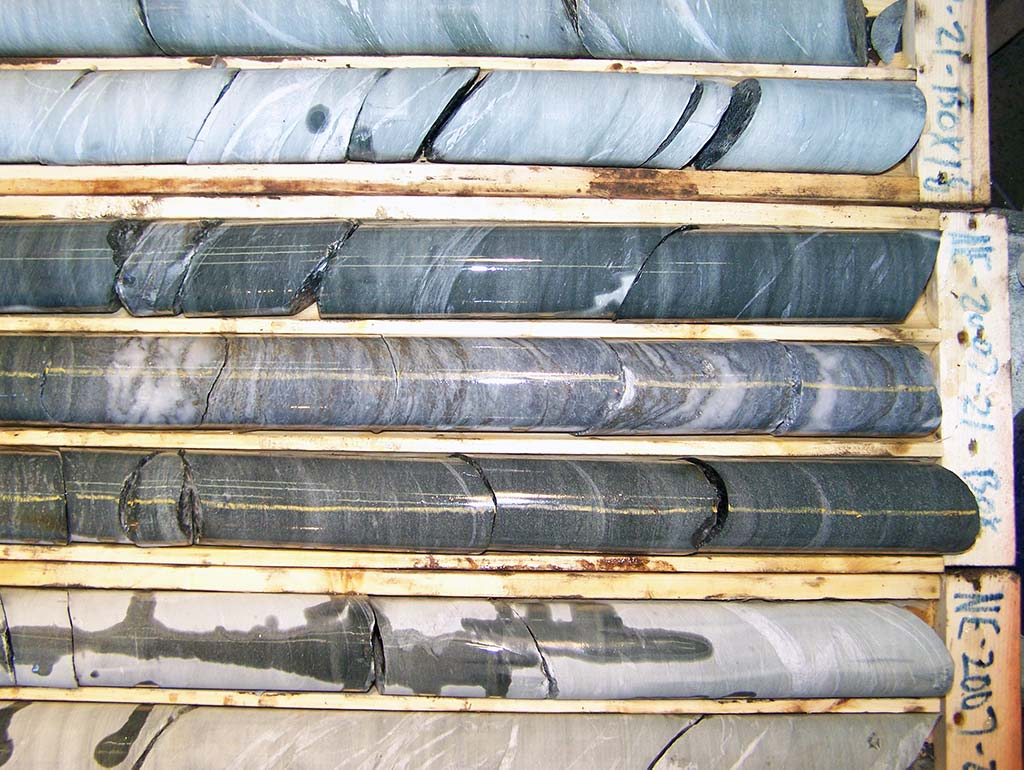
\includegraphics[width=0.8\textwidth,height=30mm]{./Capitulo_0/testemunho.jpg}	
	\caption{Testemunhos de sondagem de rochas. Amostras retiradas a partir da perfuração do solo, que apresentam uma informação contínua vertical das rochas e mineralogias presentes em uma região. }
	\label{testemunho_de_sondagem}
\end{figure}
\FloatBarrier

Desta forma, a única informação que possuímos é a informação vertical fornecida pelos testemunhos, como demonstrado na figura \ref{testemunhos_sondagem_vertical}. As decisões da mineração não podem ser estabelecidas sem o conhecimento das informações entre os furos de sondagem, que podem representar malhas espaçadas em muitos metros. A amostragem exaustiva dos depósitos minerais também é inviável economicamente, pois em alguns casos, cada metro de amostra sondada pode corresponder a um valor de \$100 a \$400 reais. 



\FloatBarrier
\begin{figure}[!htb]
	\centering
	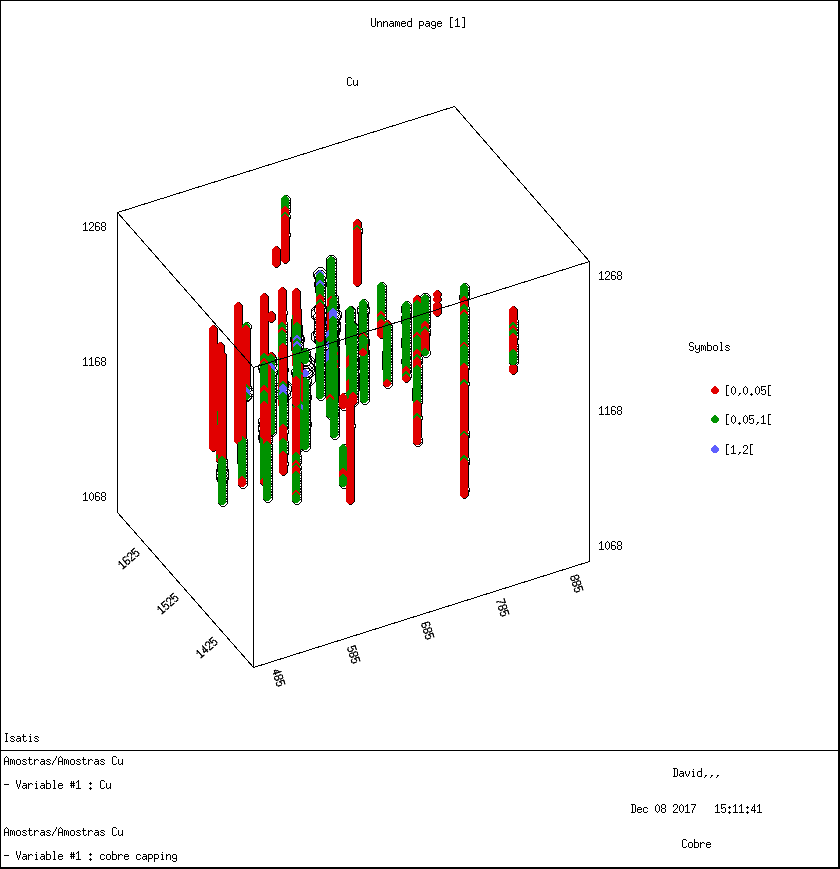
\includegraphics[scale=0.45]{./Capitulo_0/samples.png}	
	\caption{Testemunhos de sondagem representados em um software de mineração, para um depósito de cobre. }
	\label{testemunhos_sondagem_vertical}
\end{figure}
\FloatBarrier

A geoestatística é a ciência que permite a espacialização das informações obtidas em um volumes menores, para um domínio maior, de forma a permitir o planejamento e tomada de decisões na mineração, e o estudo sistemático dos corpos mineralizados. A figura \ref{simulado_teste} demonstra a espacialização dos dados obtidos na figura \ref{testemunhos_sondagem_vertical} dos testemunhos de sondagem de cobre.

\FloatBarrier
\begin{figure}[!htb]
	\centering
	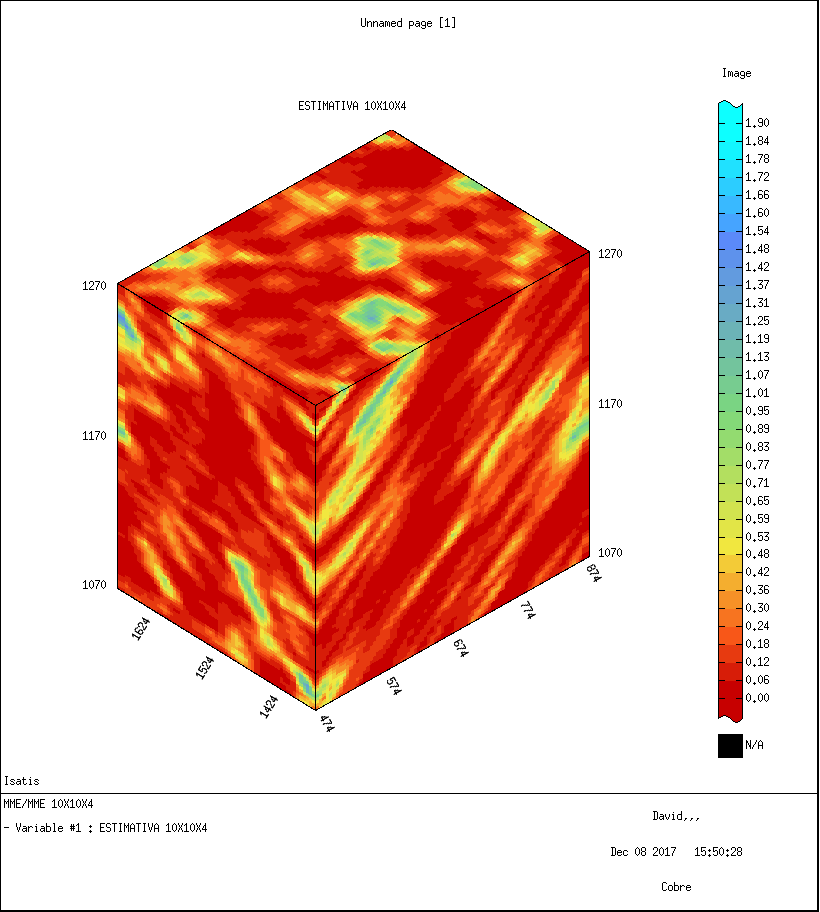
\includegraphics[scale=0.45]{./Capitulo_0/simulado.png}	
	\caption{Espacialização a partir das amostras do testemunho de sondagem obtidos na figura \ref{testemunhos_sondagem_vertical}, para um depósito de cobre. }
	\label{simulado_teste}
\end{figure}
\FloatBarrier

 A partir de um modelo espacializado é possível planejar a mineração e tomar a decisões na lavra, como a criação de \textbf{modelos econômicos}, a determinação das \textbf{cavas matemáticas}, o \textbf{sequenciamento das operações}. Segundo \citet{rossi2013mineral}, o objetivo principal da geoestatística consiste em 4 etapas principais: 
 
 \begin{enumerate}
 	\item Obtenção de amostras e administração da amostragem
 	\item Interpretação geológica e modelagem 
 	\item Interpolação dos teores
 	\item Acesso às incertezas geológicas
 \end{enumerate}

A \textbf{obtenção de amostras e administração da amostragem} consiste no conjunto de técnicas utilizada para obter uma malha de amostragem que reduza o erro obtido pela interpolação espacial das propriedades de interesse. Por exemplo, a malha de amostragem em um depósito de ferro bandado, conhecido como \textit{(Banded Iron Formations)} , pode ser dimensionada para que se reconheçam os minerais deletérios durante a fase de metalurgia. 

A \textbf{interpretação geológica e modelagem} permite reconhecer as dimensões e formas do corpo geológico e principais estruturas. Um dos grandes desafios da mineração é conseguir reconhecer os limites dos corpos minerais e sua forma. A geoestatística permite utilizar técnicas que auxiliem no reconhecimento das formas destes corpos de maneira grosseira, a partir da \textit{modelagem implícita}. O objetivo do uso destas técnicas é reduzir a quantidade de trabalho demandada pelo geólogo para que se possam produzir modelos condizentes com a realidade, e ao mesmo tempo, poupar trabalho excessivo pelo desenvolvimento de seções verticais. 

A \textbf{Interpolação de teores} consiste no objetivo principal deste livro, em que realizamos a espacialização das propriedades de interesse das amostras para um domínio espacial maior. Esta espacialização pode ser realizada para apenas uma variável (caso univariado), ou para diversas variáveis em conjunto (caso multivariado). O objetivo principal da interpolação é garantir, com maior segurança possível, que um volume direcionado da lavra para o beneficiamento mineral possua \textbf{valor esperado}, ou \textbf{valor médio}, correto. 

O \textbf{Acesso às incertezas geológicas}  pode ser realizado a partir de técnicas avançadas de geoestatística como a simulação, ou geoestatística não-linear. Pretende-se desta forma tentar reconhecer as incertezas locais de uma propriedade do depósito, e avaliar quão díspares podem ser as medições em regiões do depósito que desconhecemos. A incerteza geológica é, sem dúvida, um dos fatores que mais afetam o \textbf{risco} do empreendimento mineiro. Para que os investidores possam verificar o risco de seus investimentos, foram criados os \textbf{códigos de mineração}, que criaram padrões nomear regiões do depósito mineral com maior ou menor incerteza quanto uma propriedade de interesse, geralmente aquela de retorno econômico. 
 
 Segundo \citet{matheron1963principles}, criador da geoestatística, podemos definí-la tal como:
 
 \FloatBarrier
 \begin{remark}	
 	\textit{"Geoestatística, na sua maior aceitação, consiste no estudo da distribuição do espaço de valores úteis para engenheiros de minas e geólogos, como teores, espessura da camada, ou acumulação, incluindo as práticas mais importantes para a avaliação de depósitos minerais" - \cite{matheron1963principles}} 
 \end{remark}
\FloatBarrier

Atualmente o uso da geoestatística compreende uma diversidade enorme de áreas, desde a \textbf{engenharia civil}, \textbf{engenharia agrícola}, \textbf{engenharia ambiental}, \textbf{geografia}, \textbf{engenharia hídrica} e até mesmo em áreas que não se resumem à dados geograficamente referenciados, mas espacialmente referenciados em objetos ou seres, como a \textbf{mecânica} ou \textbf{medicina}. Podemos entender a geoestatística sob uma perspectiva mais ampla, abordando o estudo das incertezas a cerca de fenômenos temporalmente ou espacialmente localizados. O professor \citet{goovaerts1997geostatistics}, demonstra claramente a nossa dificuldade de entender as incertezas:

 \FloatBarrier
\begin{remark}	
	\textit{"A respeito da incerteza ... ela surge do nosso conhecimento imperfeito do fenômeno, dependente dos dados e ainda mais dependente do modelo, em que o modelo especifica nossas decisões (concepções) a priori do fenômeno. Nenhum modelo tal como a medida da incerteza, pode ser objetiva." - \cite{goovaerts1997geostatistics}} 
\end{remark}
\FloatBarrier

Podemos entender então as limitações acerca dos modelos geoestatísticos. Estamos sempre \textbf{dependentes das amostras recolhidas para a avaliação}, como também a escolha dos modelos que melhor representam as características de um fenômeno. A geoestatística constitui atualmente a área que melhor consegue caracterizar a incerteza geológica, dada as condições de amostragem que obtemos na mineração e de muitos problemas georeferenciados.  Definimos a geoestatística como:

\begin{definition} [Geoestatística]
	\textit{A geoestatística é a ciência capaz de transformar as informações obtidas por amostras georeferenciadas em conhecimento, a partir da caracterização da incerteza geológica, da interpretação destes dados, das inferências e estimativas, e da tomada de decisão pelo reconhecimento do fenômeno estudado.}
\end{definition}

 \section{Qual é o objeto de estudo da geoestatística?}
 
 A geoestatística é a ciência que permite o estudo de variáveis regionalizadas. O capítulo \ref{cap_var_reg} trará informações a respeito desta teoria, que compõe o objeto principal do estudo da geoestatística. Uma variável regionalizada é aquela que pode assumir um valor específico no espaço. Este valor é \textbf{determinístico}, gerado a partir de fenômenos que muitas vezes não conhecemos. Por não conseguirmos acessar as informações a respeito desta variável, optamos por utilizar uma metodologia \textbf{estocástica} para acessar a nossa \textbf{incerteza} a cerca do fenômeno que estudamos. Desta forma pensamos na variável regionalizada com um aspecto \textbf{dicotômico}, a medida que possui valor real onde conhecemos, e valor aleatório onde desconhecemos. 
 
 O físico Erwin Schrödinger desenvolveu um problema em 1935 muito similar a esta condição das variáveis regionalizadas. O experimento foi chamado de "Gato de Schrödinger". O experimento propunha que um gato fosse preso em uma caixa, com um veneno que poderia aleatoriamente ser liberado, matando o gato em seguida. Para quem observa a experiência do lado de fora, não há como detectar se o gato está vivo ou morto, logo o estado de sobrevivência do gato é indefinido, dependendo da real observação de dentro da caixa. A figura \ref{gato} demonstra este experimento. 
 
 
 \FloatBarrier
 \begin{figure}[!htb]
 	\centering
 	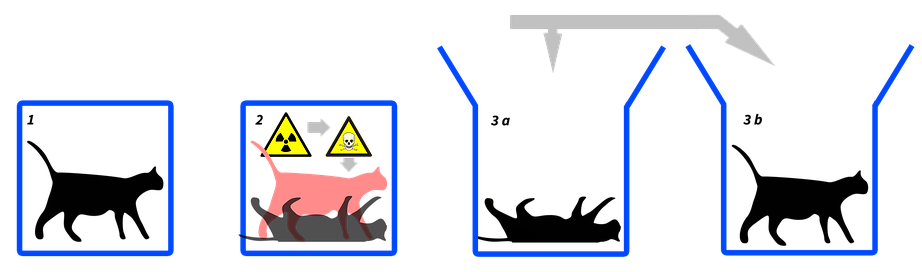
\includegraphics[scale=0.60]{./Capitulo_0/gato.png}	
 	\caption{Experiência do "Gato de Schrödinger", proposta em 1935 pelo físico Austríaco Erwin Schrödinger. 1) O gato está dentro da caixa, 2) Passado um tempo o observador externo não sabe o que está dentro da caixa. 3a) Abre-se a caixa e define-se que o gato está morto. 3) Abre-se a caixa e define-se que o gato está vivo.  }
 	\label{gato}
 \end{figure}
 \FloatBarrier
 
 Quando pensamos em termos da mineração, o problema de se definir minério ou estéril é similar ao do "Gato de Schrödinger". Não sabemos de fato o que será minerado deve ser enviado para o beneficiamento mineral, a não ser que de fato retirarmos o material do local. As \textbf{variáveis regionalizadas} funcionam de forma bem semelhante, possuindo este aspecto ao mesmo tempo determinístico e aleatório. Um depósito mineral é um evento geológico realizado durante milhões de anos. Durante o tempo de existência humana é quase impossível que estes depósitos minerais se modifiquem. Desta forma o corpo mineral, ou o "gato" já está dentro da caixa há muito tempo, porém nos é impossível determinar o seu atual estado sem que ocorra a mineração. 
 
 Ao estudar as variáveis regionalizadas, a  geoestatística propõe encontrar valores e relações que desconhecemos, sem obtermos informações diretas do depósito mineral. Considerando a variabilidade inerente destas variáveis podemos criar modelos estatísticos que possam inferir propriedades que desconhecemos em outras regiões do depósito mineral.
  

 \section{O que podemos fazer com a geoestatística?}
 
 A partir da avaliação dos depósitos minerais utilizando a geoestatística, podemos caracterizar o fenômeno espacial e quantificar as incertezas para diferentes \textbf{variáveis}. Uma variável é uma característica  de interesse de estudo no depósito mineral, que se modifica segundo seu posicionamento no espaço. No estudo da mineração possuímos uma série de diferentes tipos de variáveis associadas ao depósito mineral, tais como:
 
 \begin{enumerate}
 	\item \textbf{Químicas}: Teores de elementos químicos de interesse, ou de elementos deletérios prejudiciais no processamento mineral
 	\item \textbf{Físicas}: Dureza, densidade, condutibilidade térmica, condutibilidade hidráulica, saturação
 	\item \textbf{Geológicas}: Litologia, composição mineralógica, número de falhas, RQD (Rock quality index)
 	\item \textbf{Processamento}: Recuperação metalúrgica, recuperação mássica, moabilidade, consumo de reagentes
 	\item \textbf{Operacionais}: Resistência a penetração, consumo de explosivos, tempo de carregamento 
 	\item \textbf{Econômicas}: Preço de mercado, valor presente líquido
 \end{enumerate} 

O entendimento de cada uma destas variáveis permite a tomada de decisão de lavra de uma parte constituinte do depósito mineral. O uso de modelos geoestatísticos para cada uma destas variáveis deve, no entanto, ser específico para cada tipo de variável calculada. Neste livro introdutório abordamos principalmente os problemas que se relacionam com variáveis consideradas \textbf{aditivas}. Algumas variáveis que podem ser consideradas aditivas, e que representam o maior escopo de trabalho dos avaliadores de depósito mineral são \textbf{teor do elemento metálico}, \textbf{quantidade de metal de interesse}, \textbf{massa do minério} e \textbf{acumulação}. \citet{carrasco2008additivity} demonstra o conceito de aditividade de variáveis, expresso por: 


\FloatBarrier
\begin{remark}	
	\textit{"Quantidades consideradas aditivas são aquelas que a quantidade média é igual a média das quantidades." - \cite{carrasco2008additivity}} 
\end{remark}
\FloatBarrier

A variável teor, por exemplo, pode ser considerada uma variável aditiva, pois a média aritmética dos teores de duas regiões de mesma forma e volume é idêntico ao valor médio do teor nestas regiões. No caso da recuperação metalúrgica, por exemplo, não há possibilidade de se considerar a média aritmética como valor médio, sendo impossível utilizar a geoestatística linear para estimar valores de recuperação metalúrgica. \citet{carrasco2008additivity} ainda afirma a necessidade de variáveis aditivas para se realizar o processo de estimativa diretamente por meio da geoestatística linear clássica. 

\FloatBarrier
\begin{remark}	
	\textit{"Uma quantidade dita não aditiva, não pode modelar sua variabilidade espacial ou estimar diretamente" - \cite{carrasco2008additivity}} 
\end{remark}
\FloatBarrier

Para estimar ou avaliar variáveis ditas não-aditivas recorremos aos métodos de \textbf{geoestatística não linear} ou \textbf{simulação geoestatística}. Estes métodos não serão abordados neste volume deste livro, apenas abordaremos os conceitos primários da \textit{geoestatística linear}, que envolvem o tratamento de variáveis aditivas. No entanto, para o leitor iniciante, é importante entender que os métodos deste livro apenas se aplicam para \textbf{variáveis aditivas} e para amostra com o mesmo volume e forma, conceito denominado de \textbf{suporte amostral}. As estimativas realizadas no depósito mineral geralmente são feitas em volumes maiores, chamado de \textbf{suporte da estimativa} e compõe a chamada \textbf{unidade seletiva de lavra}. Segundo \citet{rossi2013mineral} uma unidade seletiva de lavra pode ser caracterizada como:

\FloatBarrier
\begin{remark}	
	\textit{"Mínimo volume de material ao qual o minério e o estéril podem ser separados, em função do método de lavra e da seletividade" - \cite{rossi2013mineral}} 
\end{remark}
\FloatBarrier

Podemos então discretizar o espaço em pequenos blocos, para se realizar a estimativa nestes locais. Este é chamado de \textbf{modelo de blocos}, representado na figura \ref{mod_blok}.

\FloatBarrier
\begin{figure}[!htb]
	\centering
	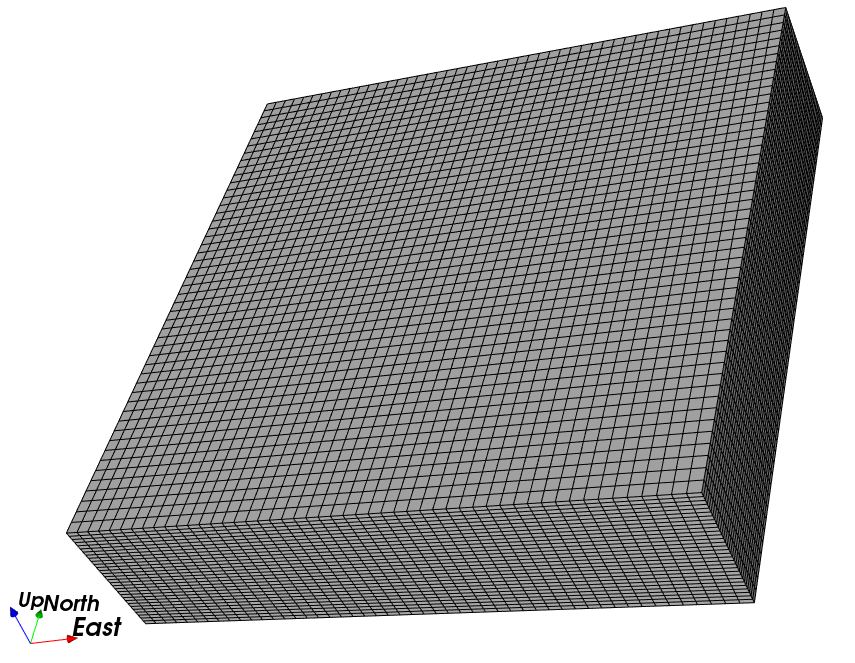
\includegraphics[scale=0.30]{./Capitulo_0/modelo_bloco.png}	
	\caption{Representação de um modelo de blocos e discretização do espaço. }
	\label{mod_blok}
\end{figure}
\FloatBarrier

Assim podemos dividir o espaço a ser estimado em pequenos volumes de decisão na lavra. Para fins de planejamento mineral, quanto menor o tamanho destes blocos, melhor a facilidade do planejamento. No entanto, para fins de avaliação de depósitos, blocos de tamanho pequeno produzem estimativas espúrias. 

O equilíbrio entre estas duas vontades deve ser encontrado para constituir o tamanho adequado da unidade seletiva de lavra. Uma das regras de ouro da mineração geralmente afirma que: \textbf{o tamanho do bloco não deve ser inferior a 1/4 do tamanho da malha de amostragem}. Esta é uma afirmação atrela o tamanho do bloco geralmente a uma malha de amostragem bem definida e calculada, o que muitas vezes não condiz com as questões práticas.

\begin{proposition}
	\textit{Segundo a regra de ouro da geoestatística um bloco estimado não deve ter tamanho inferior a 1/4 do espaçamento da malha de amostragem. Quando considerada uma malha irregular este tamanho não pode ser menor que 1/4 do valor esperado dos espaçamentos. O valor esperado pode ser calculado a partir da média aritmética dos espaçamentos.}
\end{proposition}

A discretização do depósito mineral em diferentes domínios nem sempre ocorre somente em modelos de blocos. Diferentes formas de caracterização dos volumes no espaço pode ser utilizada na geoestatística e no planejamento minera. A Figura \eqref{Modelo_blocos} demonstra alguns exemplos de divisão do espaço. Algumas delas como \textbf{polígonos de influência} e \textbf{triangulação de Delunay} representam antigas formas de estimativa de um depósito mineral, mas que, no entanto, ainda são usuais por outras formas de análise. 

\FloatBarrier
\begin{figure}[!htb]
	\centering
	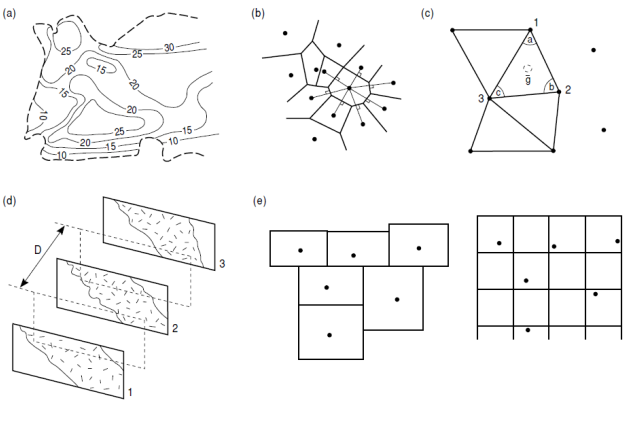
\includegraphics[scale=0.6]{./Capitulo_0/Modelo_de_blocos.png}	
	\caption{Figura demonstrando diversas apresentações de uma propriedade do depósito mineral. a) isolinhas b) Polígonos de influência c) triangulação d) seção paralelas e) blocos irregulares f) blocos regulares }
	\label{Modelo_blocos}
\end{figure}
\FloatBarrier

A partir da definição das variáveis do depósito mineral o engenheiro é capaz de estimar a viabilidade técnica e econômica do depósito mineral.  O artigo 6, do decreto 9.406 de 12 de junho de 2018 do código mineral vigente define:

\begin{definition}[Jazida Mineral]
	\textit{Toda a massa de substância mineral ou fóssil, que aflore na superfície ou já exista no solo, no subsolo, no leito ou no subsolo do mar territorial, da zona econômica exclusiva ou da plataforma continental, que tenha valor econômico}
\end{definition}


 A partir da avaliação de depósitos minerais, conseguimos então, identificar regiões econômicas e capazes do aproveitamento industrial. 


\section{Como utilizar a geoestatística?}

A geoestatística clássica utilizada neste livro não aborda conceitos matemáticos complexos, mas ainda sim constitui base para a resolução de muitos problemas de estimativa na mineração. Mesmo que os cálculos não sejam complexos, são de certa forma muito onerosos computacionalmente. As resoluções podem ser demoradas e alguns casos exigirem alta performance computacional. Desta forma, o uso de algoritmos refinados se torna cada vez mais importante nas análises geoestatísticas. 

Durante a fase de avaliação das jazidas minerais o computador exerce função essencial como ferramenta de estudo. Uma quantidade substancial de softwares estão disponíveis em meio comercial e alguns aplicativos livres também existem. Softwares comerciais são mais custosos, mas possuem suporte técnico e manutenção de seus sistemas. Apresentam código fechado ao público externo e pertencente geralmente aos proprietários. Softwares gratuitos geralmente são disponibilizados por universidades, possuem código aberto ao público e podem ser facilmente obtidos via Internet. 

Uma das bibliotecas gratuitas mais importantes é sem dúvida o GSLIB (Geostatistical Software Library) e apresenta além dos executáveis do programa seus algoritmos, escritos em Fortran 90 e disponibilizados no site. Os programas são administrados pelo doutor Clayton Deutsch e Emmanuel Schnetzler. Mais informações sobre o pacote de softwares pode ser encontrado no site \url{www.gslib.com} ou no guia de uso \cite{deutschcv1998gslib}. Neste livro abordamos nas seções A, B e C o uso dos principais softwares e linguagem R.  

O alinhamento da geoestatística com o desenvolvimento de algoritmos cria dependências com as disciplinas de programação. Os engenheiros e geólogos estão cada vez mais alinhados com o desenvolvimento de algoritmos, principalmente com as linguagem R e Python, pela sua simplicidade e facilidade de implementação.

O uso dos softwares de mineração geralmente requerem que os arquivos de dados sejam organizados eficientemente em formatos pré-estabelecidos, gerados pelas campanhas de exploração.  Essa compilação dos dados é trabalhosa e necessita de uma validação primordial, tornando o trabalho de preparação dos dados às vezes muito mais demorado que as implementações dos programas.  

Entre as aplicações mais comuns encontradas em softwares de mineração, temos:

\begin{itemize}
\item Uma grande variedade de procedimentos de avaliação dos dados (estatísticas, gráficos, etc.:)
\item Determinação da qualidade dos dados e dos protocolos de amostragem
\item Modelagem tridimensional e visualização de formas geológicas complexas e distribuição das amostras.
\item Preparação de seções planas e verticais 
\item Gráficos de contorno tanto do teor como de outras variáveis 
\item Caracterização da continuidade espacial (Variogramas automáticos, mapas de variograma, variogramas experimentais e modelagem)
\item Modelagem de blocos do depósito
\item Metodologias de cálculos de recurso e reservas
\item Avaliações dos efeitos de vários métodos de mineração
\item Determinação da viabilidade econômica de depósitos
\end{itemize}

Alguns destes softwares podem ainda incluir ferramentas de planejamento de mina, tal como otimização de cava, sequenciamento, desenho de cava, etc. A grande quantidade de ferramentas adicionadas nestes programas geralmente os tornam pouco específicos para análises espaciais, obtendo apenas algumas rotinas específicas para trabalhos mais simples. 


\section{O que a geoestatística não faz?} 

Toda ferramenta possui suas limitações. A geoestatística é a melhor ferramenta para análises espaciais até então criada, mas ela possui limitações no uso de seus modelos. Primeiramente \textbf{a geoestatística não é uma caixa preta}. Isso significa que uma boa análise do depósito mineral não depende exclusivamente de apertar um botão, como muitos modelos mais simples fazem. Para criar modelos geoestatísticos adequados eles devem passar por uma intensa avaliação e reavaliação dos parâmetros de ajuste destes modelos. 

Em segundo lugar \textbf{a geoestatística não é uma bola de cristal}. Quando realizamos estimativas estamos susceptíveis a erros e incertezas. Uma boa estimativa dos depósitos minerais propiciará redução dos erros, mas inevitavelmente não podemos sempre esperar resultados exatos. Além das condições relacionadas a escolha e refinamento dos modelos, também temos condições inerentes da incerteza geológica.  \citet{maranhao1985introduccao} demonstra a classificação de jazidas minerais no ponto de vista da avaliação de reservas, identificando quatro grupos principais: 

\begin{enumerate}
	\item \textbf{Grupo 1}. Pertence aos depósitos estratiformes, cujos representantes típicos são as jazidas sedimentares de origem marinha, que possuem grandes dimensões, forma mais ou menos constante, e regularidade na distribuição de teores.  Também  incluem neste grupo as jazidas metamórficas de ferro, tais como nos depósitos do quadrilátero ferrífero. Também apresenta alguns depósitos de disposição horizontal ou a subhorizontal como jazidas de calcário, carvão, sais, gipsita e alguns depósitos para construção civil, como gnaisses e granitos.
	\item \textbf{Grupo 2}. O segundo grupo apresenta corpos minerais interrompidos ou levemente interrompidos e uma distribuição mais irregular dos teores que do primeiro grupo. Estas representam as jazidas de alteração superficial como depósitos de níquel e bauxita, depósitos com pequenas intrusões alcalinas, como carbonatitos e sienitos, jazidas de rochas ultrabásicas e hidrotermais.
	\item \textbf{Grupo 3} O terceiro grupo geralmente enquadra jazidas de forma variável e mineralização muito irregular, compondo os principais depósitos auríferos, platinoides e diamantes. Também aborda os depósitos de veios polimetálicos e depósitos de forma lenticular, como de cobre e níquel. 
	\item \textbf{Grupo 4} Representa o grupo mais irregular de todos, compondo pegmatitos de pedras preciosas, alguns veios hidrotermais com metais raros e nobres e algumas jazidas ultrabásicas de platina e diamante. 
\end{enumerate}

Quanto maior a irregularidade do depósito e heterogeneidade de suas propriedades, maior será a dificuldade dos modelos geoestatísticos de predizerem com exatidão os resultados. Dependendo da \textbf{continuidade espacial} da propriedade e da sua \textbf{dispersão}, a aplicação de modelos simples ou complexos simplesmente não altera o nosso conhecimento sobre a \textbf{incerteza geológica}, pois a complexidade do depósito mineral é tão grande, e as amostragens realizadas em tão pouca quantidade, que se torna mais fácil jogar uma moeda para cima para decidir se devemos ou não lavrar um depósito. Neste caso, quando os métodos geoestatísticos falham, é necessário rever as metodologias de amostragem, e tentar encontrar soluções que simplifiquem as variáveis do problema. 

Desta forma a geoestatística também tem outra limitação: \textbf{Os modelos geoestatísticos requerem amostras realizadas em quantidade e qualidade adequada para gerar resultados satisfatórios}. Esta talvez seja uma das limitações mais difíceis de se conseguir abordar dentro da mineração. Para estimar de forma adequada precisa-se de amostras, e amostras são caras. Muitas empresas deixam de amostrar adequadamente seus depósitos minerais com finalidade de redução de custos, mas acabam por avaliar mal seus depósitos minerais, e consequentemente, obtém baixo lucro ou inviabilizam o uso sustentável dos recursos minerais. O termo qualidade, também é uma questão muito importante. Muitas vezes as amostragens realizadas possuem protocolos mal dimensionados. Alguns métodos de amostragem de jazidas também devem ser conduzidos de forma bem precisa para realizarem estimativas adequadas, mas apesar de ser uma das etapas mais importantes na mineração, as empresas muitas vezes colocam a tarefa nas mãos de profissionais pouco qualificados. 


\section{Questões éticas na avaliação de depósitos minerais} 

Avaliar depósitos minerais é uma atividade incerta, devido a natureza dos depósitos minerais, no entanto, não há justificativa para o mal uso das técnicas, nem ao mesmo para decisões arbitrárias que não envolvam decisões puramente lógicas ou racionais. Infelizmente o setor mineral acaba por ser alvo de pessoas com má conduta, por ser uma área de grandes riquezas. Esta não é, com certeza, a personalidade da grande maioria dos trabalhadores que se dedicam diariamente no setor mineral, mas pessoas acabam por utilizar a justificativa do "incerto" para vender depósitos minerais subvalorizados. Um avaliador de depósitos minerais deve realizar sua tarefa friamente, analisando a viabilidade do depósito independente se ele gerará riquezas ou não. 

É importante também para os gestores e gerentes de minas entenderem a natureza do problema, e que as incertezas geológicas produzirão muitas vezes resultados diferentes dos pretendidos. A mineração trata do aproveitamento de recursos que são limitados pelo tempo geológico de sua criação. Enquanto o ser humano ainda não controlar o tempo, é indiscutível que temos de aproveitar os recursos minerais existentes da melhor forma que consigamos. A avaliação de depósitos minerais é o alicerce das decisões na mineração, por isso é impreterível que os processos sejam realizados de forma mais correta possível. 

\begin{proposition}
	\textit{Está nas mãos do avaliador de depósitos minerais a determinação das condições necessárias para a progressão da lavra. O desenvolvimento de seus projetos deve seguir sempre com conhecimento e idoneidade, pois é dele que deriva o trabalho de pessoas, o aproveitamento correto dos recursos minerais e da sociedade que aproveita estes recursos}
\end{proposition}

\section{Alguns conceitos iniciais sobre jazidas minerais}

Apresentamos nesta seção alguns dos principais conceitos de engenharia de minas, necessários para a realização de trabalhos de geoestatística e avaliação de depósitos no setor mineral. Apesar deste livro possuir foco na geoestatística, consideramos adequado entender conceitos gerais da mineração, que influenciam nas decisões tomadas pela avaliação dos depósitos.

\subsection{Minério} 

A definição de minério talvez seja uma das mais importantes na produção mineral. A sua determinação permite o aproveitamento econômico dos recursos minerais, decidindo o que deve ou não ser lavrado e aproveitado. Segundo \citet{hustrulid2006open}, a definição de minério pode ser considerada como:

\begin{remark}
	\textit{"Um agregado mineral com um ou mais sólidos minerais aos quais podem ser minerados, ou dos quais um ou mais produtos minerais podem ser extraídos com lucro".  \citet{hustrulid2006open}}
\end{remark}

Isto significa que nem em todas as ocasiões um minério será extraído com a finalidade de se obter lucro pela venda. Em alguns casos, as questões econômicas da extração mineral podem ser contra intuitivas neste sentido, devido a políticas externas, estados de guerra, monopolização da produção, entre diversos outros fatores. Neste caso preferimos adotar o conceito de minério a partir do seu benefício, nem sempre ele sendo econômico. Definimos minério como: 

\begin{definition}[Minério]
	\textit{Minério é todo agregado mineral ou fóssil cabível de aproveitamento técnico, que possibilita um benefício, seja ele econômico ou social, de forma a propiciar os interesses das diferentes componentes da sociedade, sejam elas a União, as forças sociais ou mineradores.}
\end{definition}

Um exemplo bem característico de minérios explotados contra o senso econômico são os minerais radioativos, de monopólio da União. É de interesse estratégico de um país deter estes recursos capazes de produzir energia e armas, sendo muitas vezes gastos valores acima do valor do minério para sua extração. 


\subsection{Teor de corte e teor crítico}

O conceito de teor de corte (ou cutoff) é definido como aquele em que o valor do conteúdo metálico ou mineral, em um certo volume de rocha, permite sua extração econômica. Os teores de corte são usados para distinguir blocos de minério e estéril em vários estágios da evolução da estimativa da jazida mineral (exploração, desenvolvimento e produção). O teor crítico, no entanto, representa o teor ao qual se delimita o limite entre prejuízo e lucro. \citet{rendu2014introduction} define o teor de corte como:


\begin{remark}
	\textit{"O teor de corte geralmente é definido como a mínima quantidade de um produto de valor ou metal que em uma tonelada métrica deve conter para que este material seja enviado para a planta de beneficiamento"} - \cite{rendu2014introduction}
\end{remark}

\subsection{Continuidade}

A continuidade é um termo derivado em toda a história da matemática e da ciência desde tempos remotos. Talvez uma das primeiras concepções da continuidade seja com o pardoxo de Zenão, que conta a história da corrida de Aquiles e a tartaruga. \citet{srivastava1989robust} demonstram o sentido da continuidade como: 

\begin{remark}
	\textit{"Uma descrição da similaridade ou da dissimilaridade entre pares de valores com uma função de sua speração do vetor h"} - \cite{srivastava1989robust}
\end{remark}

Em outras palavras podemos dizer que a continuidade espacial é representada pela similaridade entre medidas que se localizam em regiões diferentes no espaço. Os fenômenos geólogicos, neste caso, apresentam uma importante característica derivada de suas gêneses: Na maioria dos casos, medidas de propriedades realizadas mais próximas tendem a ser mais similares entre si do que medidas realizadas em grandes distâncias. Caracterizar a similaridade dos fenômenos geológicos é a chave para garantir que as estimativas e a caracterização da incerteza geológicas possam ser realizadas. 

\begin{definition}[Continuidade espacial]
	\textit{Definimos a continuidade espacial como a regularidade com que uma propriedade é medida em amostras aproximadas no espaço. Se as diferenças entre as amostras for pequena, dizemos que o material é contínuo ou similar. Quando o material é muito diferente de amostras pouco espaçadas dizemos que ele é discreto ou dissimilar. Na geoestatística definimos a continuidade a partir de uma direção do espaço, podendo ela se apresentar diferencialmente de acordo com a direção adotada.}
\end{definition}

\subsection{Diluição}

Segundo \citet{susaeta2008dilution} a diluição se refere ao estéril que não é separado do minério durante a operação da lavra. Este estéril é misturado com o minério e enviado para a usina de beneficiamento. Enquanto aumenta  a quantidade de material enviado para a usina a diluição diminui o teor que deveria ser estimado e enviado para a usina corretamente. A estimativa de depósitos minerais é realizada desconsiderando os efeitos de produção e planejamento. Isto significa que os valores realmente lavrados não correspondem aos volumes planejados e induzem diferenças naturais da estimativa. O processo de comparação entre os valores reais obtidos na usina e os valores estimados pode ser definido como \textbf{aderência do planejamento de lavra} 

\begin{definition}[Aderência de lavra]
	\textit{Aderência do planejamento de lavra é todo o processo de comparação entre os valores estimados do depósito mineral e os obtidos durante a operação, seja durante a mineração, ou dos valores obtidos durante o beneficiamento mineral.} 
\end{definition}

As incertezas geológicas presentes no depósito mineral, ou as diferenças do planejamento da operação podem trazer discordâncias quanto os volumes e qualidade do material estimado e realmente lavrado, causando diluição do minério. Existem diferentes tipos de diluição durante a extração mineral. A \textbf{diluição interna} ocorre quando existem partes de estéril dentro do volume estimado do minério. Algumas vezes a amostragem pode não computar veios ou lentes de estéril dentro do bloco de decisão de lavra, dado que o volume das amostra é muito inferior ao volume das amostras. A \textbf{diluição externa} ocorre quando o planejamento mineral aborda parte do material não definido como minério, o que é comum nas regiões de contato do corpo geológico. Também há a chamada \textbf{diluição operacional}, que ocorre quando o desmonte de rochas realiza a fragmentação em regiões acima do planejado ,chamado de \textit{overbreak}, ou abaixo do planejado, chamado de \textit{underbreak}.

\subsection{Recursos e reservas minerais}

A definição de recursos e reservas minerais são alternativas para publicidade de declarações públicas relativo às incertezas geológicas do depósito mineral. A CBRR (Comissão Brasileira de Recursos e Reservas) identifica a declaração pública como:

\begin{definition}[Declaração pública]
	\textit{Declarações públicas são preparadas para informar investidores ou potenciais investidores e seus conselheiros sobre os resultados da exploração, recursos minerais ou reservas minerais. Elas incluem, mas não se limitam, a relatórios anuais ou trimestrais das entidades, notas  à imprensa, memorandos informativos, documentos técnicos, publicações em website e apresentações públicas.} 
\end{definition}

A partir de declarações públicas, as empresas podem indicar os volumes de metais e de massas estimados com base no conhecimento da incerteza geológica. Esta alternativa foi criada na década de 70, principalmente após o escândalo da empresa Bre-X, após constatado salgamento das minas de ouro em Busang na Indonésia. Definindo \textbf{Recursos} e \textbf{Reservas} minerais, o minerador classifica seus potenciais de produção segundo a incerteza geológica. A CBRR também define Recurso Mineral como:

\begin{definition}[Recurso Mineral]
	\textit{Um Recurso Mineral é uma concentração ou ocorrência de material sólido de interesse econômico dentro ou na superfície da crostra terrestre onde forma, teor ou qualidade e quantidade que apresentem perspectivas razoáveis de extração econômica.} 
\end{definition}

A definição de Recurso está ligada diretamente ao conhecimento da incerteza geológica. Os códigos de mineração não definem as técnicas necessárias para se definir os volumes de depósito de acordo com estas incertezas, apenas indicam que deve-se usar alguma técnicas pertinente para isto. A responsabilidade desta definição cai diretamente à pessoa competente responsável pela auditoria. Estes Recursos minerais podem ser divididos em ordem crescente de confiabilidade geológica de acordo com as categorias de Inferido, Indicado e Medido. A CBRR também define Reserva Mineral como

\begin{definition}[Reserva Mineral]
	\textit{Uma Reserva Mineral é a parte economicamente lavrável de um Recurso Mineral Medido e/ou Indicado. Isso inclui diluição e perdas que podem ocorrer quando o material é lavrado ou extraído e é definido apropriadamente pelos estudos nos níveis de Pré-Viabilidade ou de Viabilidade que incluem aplicação de Fatores modificadores.} 
\end{definition}

Ou seja, para transformar um recurso em reserva mineral é necessário que se prove a viabilidade da extração do minério, seja ela econômica, social, ambiental ou política. Isto é realizado a partir dos fatores modificadores.  A CBRR também define os fatores modificadores como: 


\begin{definition}[Fatores Modificadores]
	\textit{Fatores Modificadores são considerações usadas para converter Recursos Minerais em Reservas Minerais. Esses incluem, mas não se limitam a considerações sobre:  a lavra, o processamento, a metalurgia, a infraestrutura, a economicidade, o mercado, os aspectos legais, ambientais, sociais e governamentais} 
\end{definition}

As Reservas Minerais podem se dividir em provável, quando medida a partir de um Recurso Indicado e, em algumas circustâncias de um Recurso medido. A reserva provada é aquela que possui alta confiabilidade, representando recursos medidos. A figura \ref{Recursos_Reservas} demonstra graficamente os resultados da exploração mineral em recursos e rservas minerais, também apresentando sua forma de conversão, de acordo com o conhecimento geológico e os fatores modificadores.

\FloatBarrier
\begin{figure}[!htb]
	\centering
	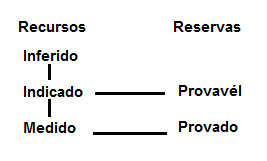
\includegraphics[scale=0.75]{./Capitulo_0/Recursos_Reservas.png}	
	\caption{Figura demonstrado a classificação de jazidas em recursos e reservas. Linhas indicando a transição entre as classificações }
	\label{Recursos_Reservas}
\end{figure}
\FloatBarrier


\subsection{Precisão e Exatidão}


Uma das premissas utilizadas na geoestatística clássica é que os resultados das amostras obtidas é um valor fixo. Esta afirmação na maioria dos casos não é realista, pois as amostragens na mineração podem apresentar diferentes valores referentes aos erros de amostragem. 

\begin{proposition}
	\textit{Para os processos de geoestatística clássica, os valores das amostras georeferenciados são determinísticos, a medida que apresentam volume, posicionamento e propriedades constantes. Isto não se aplica a todos os métodos geoestatísticos como o KVME (Kriging with Measurement Error Variance) \cite{delhomme1978applications}}
\end{proposition}


Esta variação das amostras quanto ao valor esperado por elas pode ser definido por duas propriedades: \textbf{Exatidão} e \textbf{Precisão}.  A Exatidão pode ser exemplificado como a proximidade de uma estimativa com a realidade, enquanto precisão é a medida da dispersão entorno de uma estimativa. Analogamente a precisão e a exatidão podem ser comparadas com um jogo de dardos como na figura \eqref{exat_prec}, em que pretendemos atingir o centro do alvo. Quanto mais próximo forem os disparos do centro, melhor será a sua exatidão, e quanto mais próximos forem os disparos entre si, significa que são mais precisos. Disparos podem ser precisos, no entanto, não exatos. Disparos podem ser exatos por se localizarem em média próximos do centro, mas podem ser imprecisos se distanciarem entre si. 

\FloatBarrier
\begin{figure}[!htb]
	\centering
	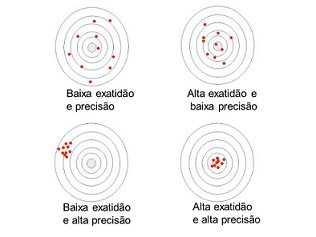
\includegraphics[scale=1.4]{./Capitulo_0/exat_prec.jpg}	
	\caption{Figura demonstrando os conceitos de exatidão e precisão. O centro do alvo é o valor verdadeiro que pretende-se alcançar com os disparos. Disparos entorno do centro são considerados exatos. Disparos próximos aos outros são considerados precisos }
	\label{exat_prec}
\end{figure}
\FloatBarrier

A amostragem na mineração ainda sofre um outro problema, quanto a reprodutibilidade, Na verdade este é um problema para a maioria dos fenômenos espaciais, pois quando amostramos uma região não há como amostrar novamente, pois estas amostras geralmente são \textbf{destrutivas}. Além disso, ao amostrar em um local específico, uma amostra mesmo que próxima já se configura como uma amostra diferente. Os trabalhos do professor \citet{gy2012sampling} invocam os principais conceitos e teorias a respeito da amostragem a granel, utilizada na mineração.

Eventualmente diversos fatores podem causar as variações e erros na amostragem. Há vários tipos de erros potenciais na estimativa de reservas minerais incluindo:

\begin{itemize}
	\item Erro de amostragem 
	\item Erros de análise química.
	\item Erros de densidade (É comum em muitos casos considerar a densidade do material constante ao longo do depósito)
	\item Erros da geologia, durante as fases de determinação da continuidade espacial e geometria do depósito mineral.
	\item Na escolha do método de lavra adotado que pode não atender as questões de seletividade do minério e estéril de forma ótima.
	\item A diluição do minério com a encaixante.
	\item Erro humano (inserção de valores errados no banco de dados, de casas decimais, et.)
	\item Fraude ( salgamento de amostras, substituições de amostras, dados não representativos, etc.)
	
\end{itemize}


\section{Conclusões} 

Neste capítulo inicial apresentamos os principais conceitos relacionados à geoestatística e ao planejamento de mina. Definimos o que é esta ciência que será abordada ao longo de todo o livro, o que ela pode realizar ou não, e sua importância dentro do contexto da mineração. Entendemos que a geoestatística é uma ferramenta para auxiliar na compreensão do desconhecido, e que é inerente ao empreendimento mineral, pois raras são as alternativas ao qual possuímos informação sistemática ao longo de todo o depósito mineral.


\section{Exercícios}
\begin{exercise} 
	Segundo a definição de \citet{carrasco2008additivity}, sabemos que uma variável é aditiva se o seu valor médio é igual a média de seus valores. Discutimos ao longo do texto que as variáveis teor e conteúdo metálico são variáveis aditivas, capazes de serem utilizadas nos modelos clássicos que abordamos neste livro. Desta forma identifique variáveis na mineração que podem ser consideradas aditivas ou não.

\end{exercise}
\begin{exercise}
	Realize um "brainstorm" e pense todas as possibilidades que podem sofrer uma mina que possam tornar um minério em um estéril. Por exemplo, a descoberta de uma outra jazida de uma empresa concorrente mais próximo do mercado consumidor pode aumentar o preço do minério e tornar parte do recurso inutilizável por um tempo. E quais seriam os fatores que fazem um estéril se tornar minério? 
\end{exercise}
\begin{exercise}
	Pretende-se determinar se uma unidade seletiva de lavra é um minério ou estéril. O custo fixo de extração do material é 5 um/ton. O custo de mineração por tonelada movimentada é 2 um/ton. A relação estéril/minério é 3/2. A Recuperação metalúrgica é de 95\% e o preço do minério é de 100 um/ton. O teor do elemento útil do bloco é 2\%. 
\end{exercise}

\begin{exercise}

Os dados da tabela seguinte demonstram um conjunto de valores estimados e dados reais obtidos. Determine:

a) O viés das estimativas. (Diferença entre a média dos valores estimados e a dos reais)

b) Considere o cut-off como 2g/ton. Determine: A proporção dos valores estimados como minério que realmente são minério. A proporção dos valores estimados como estéreis que realmente são estéreis. 

	\begin{tabular}{lllll}
		\hline
		Estimados & Real &  &  &  \\ \hline
		2.05      & 2.0  &  &  &  \\
		2.03      & 2.02 &  &  &  \\
		1.01      & 1.32 &  &  &  \\
		2.31      & 3.45 &  &  &  \\
		3.02      & 1.02 &  &  &  \\
		2.76      & 2.19 &  &  &  \\
		3.08      & 4.01 &  &  &  \\
		3.74      & 3.67 &  &  &  \\
		1.02      & 1.43 &  &  &  \\
		1.00      & 1.01 &  &  &  \\
		2.03      & 1.05 &  &  &  \\ \hline
	\end{tabular}
\end{exercise}


